\subsection{SURF - Speeded Up Robust Feature}

Segundo \cite{SURF}, em compara��o com o algoritmo SIFT que aproxima LoG por Diferencas de Gaucianas(DoG), 
SURF vai um pouco mais al�m e aproxima LoG de Box-type Filter como mostrado na
figura~\ref{fig:surf01} e n�o � utilizado nenhum tipo de suaviza��o entre
escalas , o que garante mais agilidade nos resultados porque a convolu��o com box filters s�o muito mais r�pidos com o uso de
 integral images e pode ser paralelizado

\begin{figure}[h!]
\centering
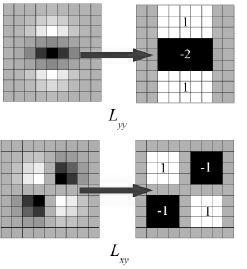
\includegraphics[scale=1.0]{images/SURF01}
\caption{Box Filtering}
\label{fig:surf01}
\end{figure}

Em geral SURF se apresenta cinco vezes mais r�pido do que DoG.